\section{Hidden extensions and latent covers}
\label{sec:hidden}

The preceding sections identify what empirical equivalence preserves. Related identifiability results show that latent representations require additional assumptions to become unique \parencite{Teicher1963,Allman2009,Locatello2019,Hyvarinen2019,Khemakhem2020}; the construction below gives a deterministic set-level witness tailored to the present observer interface. This section constructs models that share all empirically preserved information while differing in latent structure.

\subsection{Duplicate and hidden factor extensions}

Let \(\Model=(X_\Model,\pi_\Model)\) be a generative model.

\begin{definition}[Hidden factor extension]
For an inhabited set \(H\), define the hidden factor extension \(\Model^H\) by
\[
X_{\Model^H}=X_\Model\times H
\]
and
\[
\pi_{\Model^H}(x,h)=\pi_\Model(x).
\]
\end{definition}
The observation is independent of the hidden coordinate. Choosing a fixed anchor \(h_0\in H\) gives a surjective projection
\[
p:X_\Model\times H\to X_\Model,
\qquad
p(x,h)=x.
\]
The projection satisfies
\[
\pi_{\Model^H}(x,h)=\pi_\Model(p(x,h)).
\]

\begin{figure}[tbp]
\centering
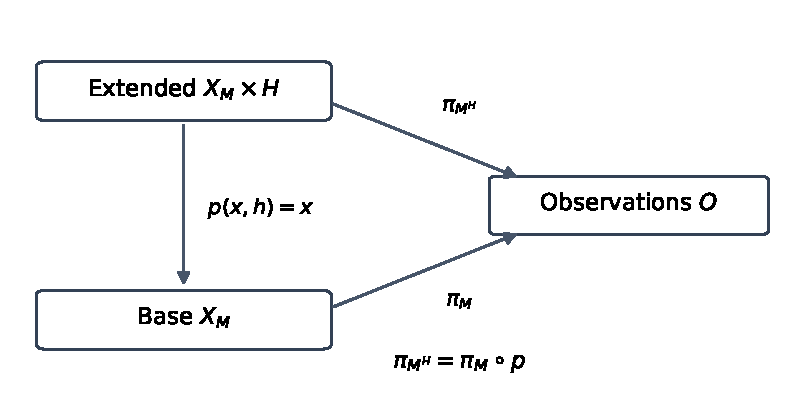
\includegraphics[width=0.84\textwidth]{figures/concept_hidden_extension.pdf}
\caption{Hidden factor extension and observation preserving projection. The projection is surjective. Distinct hidden values attached to one base state create distinct extended states with one common observation.}
\label{fig:hiddencover}
\end{figure}

\begin{theorem}[Hidden extensions preserve empirical equivalence]
For every inhabited \(H\),
\[
\Obs(\Model^H)=\Obs(\Model).
\]
Therefore \(\Model^H\approx\Model\).
\end{theorem}

\begin{proof}
Every extended observation has the form \(\pi_{\Model^H}(x,h)=\pi_\Model(x)\), so \(\Obs(\Model^H)\subseteq\Obs(\Model)\). Conversely, choose an anchor \(h_0\in H\). For every \(x\in X_\Model\), the extended state \((x,h_0)\) produces \(\pi_\Model(x)\). Hence \(\Obs(\Model)\subseteq\Obs(\Model^H)\).
\end{proof}
\begin{corollary}[Experimental invariance of hidden extensions]
For every admissible experiment \(e\),
\[
\Out_e(\Model^H)=\Out_e(\Model).
\]
\end{corollary}
\begin{theorem}[Hidden collisions]
If \(H\) contains distinct values \(h_0\neq h_1\) and \(X_\Model\) contains \(x\), then
\[
(x,h_0)\neq(x,h_1)
\]
but
\[
\pi_{\Model^H}(x,h_0)=\pi_{\Model^H}(x,h_1).
\]
Therefore the extended observation map is noninjective and \(\Model^H\) has no exact latent decoder.
\end{theorem}

\begin{proof}
The ordered pairs are distinct because their second coordinates differ. Both observations reduce by definition to \(\pi_\Model(x)\). The observation map is therefore noninjective. Exact latent decoding would imply injectivity, which is impossible.
\end{proof}
The Boolean extension uses \(H=\bool\). The duplicate model is the same two copy construction written as a specific finite hidden factor.

\subsection{Finite hidden multiplicity}

For a positive integer \(m\), define
\[
X_{\Model^{(m)}}=X_\Model\times\{0,1,\ldots,m-1\}
\]
and ignore the second coordinate during observation. Each base latent state generates \(m\) extended states in one observation fiber.

\begin{proposition}[Arbitrary finite hidden families]
For every base state \(x\in X_\Model\), the map
\[
\iota_x:\{0,\ldots,m-1\}\to X_{\Model^{(m)}},
\qquad
\iota_x(j)=(x,j),
\]
is injective, and every state in its image produces \(\pi_\Model(x)\).
\end{proposition}
Thus finite latent multiplicity can be increased without changing reachable observations or any admissible outcome set. In the verified source, \texttt{finiteMultiplicityModel M n} uses the hidden type \(\operatorname{Fin}(n+1)\); the paper parameter \(m\) is therefore \(n+1\).

\subsection{Countable hidden multiplicity}

The construction is not restricted to finite hidden sets. Let
\[
X_{\Model^{(\mathbb N)}}=X_\Model\times\mathbb N
\]
and define
\[
\pi_{\Model^{(\mathbb N)}}(x,n)=\pi_\Model(x).
\]
For each \(x\), the map \(n\mapsto(x,n)\) embeds \(\mathbb N\) into the observation fiber over \(\pi_\Model(x)\). The model remains empirically equivalent to \(\Model\), and every admissible outcome set remains equal. If \(X_\Model\neq\varnothing\), distinct natural number coordinates give a collision, so exact latent decoding is impossible.

This result separates empirical class size from latent fiber size. An empirical class can contain representatives with one, finitely many, or countably many latent states above the same accessible observation.

\subsection{Latent covers}

The product construction is one example of a more general relation.

\begin{definition}[Latent cover]
An extended model \(\Extended\) is a latent cover of a base model \(\Model\) when there exists a surjective projection
\[
p:X_{\Extended}\to X_\Model
\]
such that
\[
\pi_{\Extended}(z)=\pi_\Model(p(z))
\]
for every \(z\in X_{\Extended}\).
\end{definition}
Latent covers compose. The identity map makes each model a cover of itself.

\begin{theorem}[A latent cover is empirically equivalent to its base]
If \(\Extended\) covers \(\Model\), then
\[
\Obs(\Extended)=\Obs(\Model).
\]
Consequently, every admissible experiment has the same possible outcomes under both models.
\end{theorem}

\begin{proof}
Observation preservation shows that every observation of \(\Extended\) is an observation of \(\Model\). Surjectivity shows that every base latent state has an extended preimage, and observation preservation gives the same accessible output. Hence the reachable sets are equal. Outcome equality follows from \Cref{thm:outcomeinvariance}.
\end{proof}
\begin{definition}[Strict latent cover]
A latent cover is strict when its projection \(p\) is noninjective.
\end{definition}
A strict cover contains distinct extended states that project to one base state. Observation preservation then forces those extended states to share one observation.

\begin{theorem}[Strict covers prevent exact latent reconstruction]
If \(\Extended\) is a strict latent cover of \(\Model\), then \(\pi_{\Extended}\) is noninjective and \(\Extended\) has no exact latent decoder.
\end{theorem}

\begin{proof}
Since the projection is noninjective, choose \(z_1\neq z_2\) with \(p(z_1)=p(z_2)\). Observation preservation gives
\[
\pi_{\Extended}(z_1)
=\pi_\Model(p(z_1))
=\pi_\Model(p(z_2))
=\pi_{\Extended}(z_2).
\]
Thus the extended observation map is noninjective. Exact decoding is therefore impossible.
\end{proof}
\subsection{Existence of strict covers for inhabited models}

Every inhabited model has a Boolean strict hidden extension. The construction can then be repeated.

\begin{theorem}[Every inhabited model admits a strict latent cover]
For every generative model with at least one latent state, there exists an empirically equivalent strict latent cover with additional latent distinctions.
\end{theorem}

\begin{proof}
Use the Boolean hidden extension. Projection onto the base state is surjective and observation preserving. The two Boolean values make the projection noninjective.
\end{proof}
The Lean predicate \texttt{LatentlyMaximal} means that no strict latent cover exists. The theorem negates that predicate for every inhabited model. This definition is not ordinary maximality in a partial order. A strict cover means a noninjective surjective projection; for infinite models such a projection may be a self-map. For example, \(X=\mathbb N\), \(O=\{0\}\), and \(\pi(n)=0\) admit the strict self-cover \(p(n)=\lfloor n/2\rfloor\). Surjectivity follows from \(p(2n)=n\), and \(p(0)=p(1)\) proves noninjectivity. Additional hidden labels also need not increase an infinite set's cardinality. The proved conclusion is the existence of strict covers within the specified model class. It does not assert a physically realized hierarchy of hidden variables.
